% =====================================================================
%  Frame "Systolic array" : figure de Kung (1982) + produit matriciel
%  + tableau systolique 2D (frames extraites de systolic_gif.gif).
%  Remplace la frame systolic d'origine.
% =====================================================================
\begin{frame}
\frametitle{Edge TPU}
\framesubtitle{Systolic array}

\begin{center}
{\scriptsize
$\underbrace{\begin{bmatrix} w_{11} & w_{12} & w_{13}\\
                             w_{21} & w_{22} & w_{23}\\
                             w_{31} & w_{32} & w_{33}\end{bmatrix}}_{\mathbf{W}\ \text{weights, held in the PEs}}
 \times
 \underbrace{\begin{bmatrix} a_{11} & a_{12} & a_{13}\\
                             a_{21} & a_{22} & a_{23}\\
                             a_{31} & a_{32} & a_{33}\end{bmatrix}}_{\mathbf{A}\ \text{activations, streamed in}}
 =
 \underbrace{\begin{bmatrix} c_{11} & c_{12} & c_{13}\\
                             c_{21} & c_{22} & c_{23}\\
                             c_{31} & c_{32} & c_{33}\end{bmatrix}}_{\mathbf{C}\ \text{partial sums, flow down}}$}
\end{center}

\vspace{0.05cm}

\begin{minipage}{0.40\textwidth}
\begin{center}
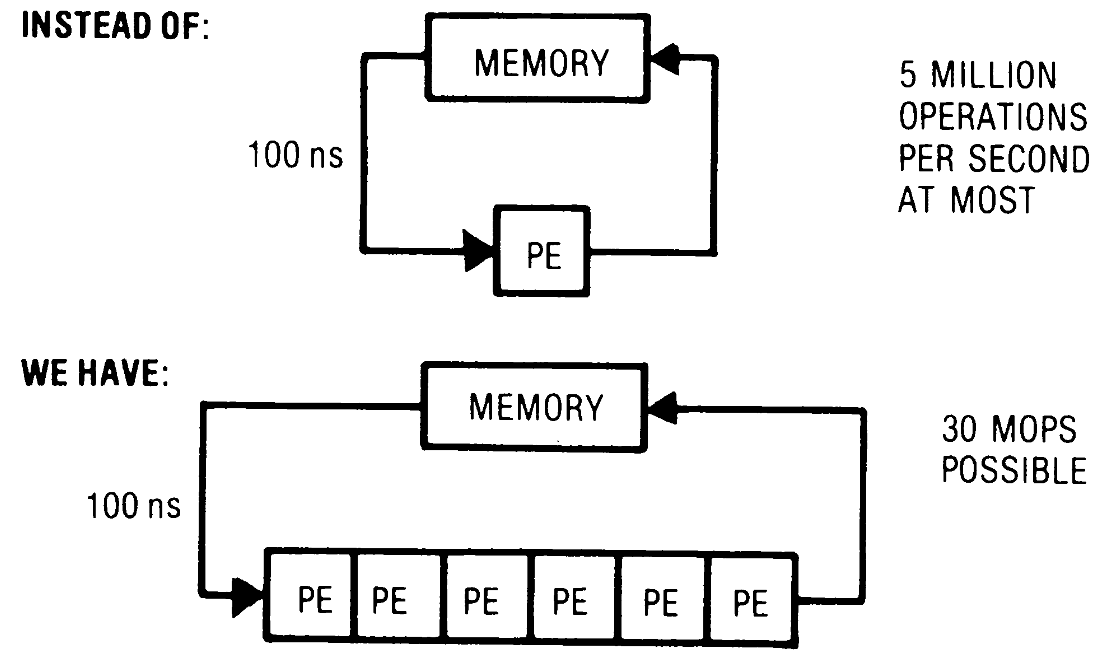
\includegraphics[width=\linewidth]{systolic_array.png}\\[2pt]
{\tiny H.\,T. Kung, \emph{Why systolic architectures?} (1982)}
\end{center}
\end{minipage}\hfill
\begin{minipage}{0.57\textwidth}
\begin{center}
\only<1>{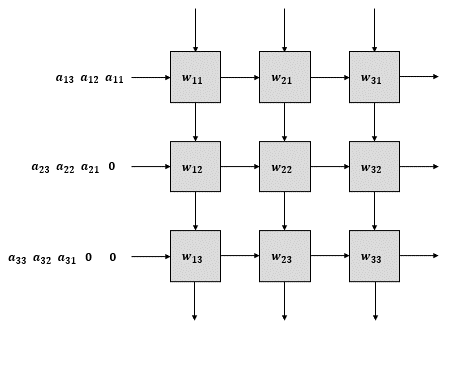
\includegraphics[height=4.1cm]{bench/img/sys_1.png}}%
\only<2>{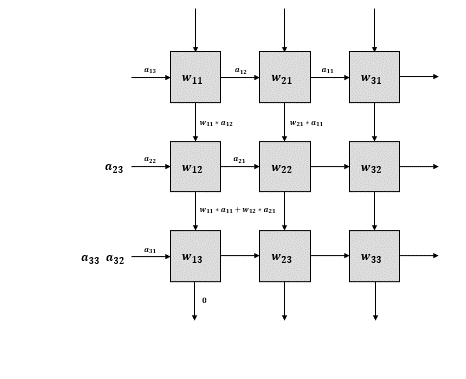
\includegraphics[height=4.1cm]{bench/img/sys_4.png}}%
\only<3>{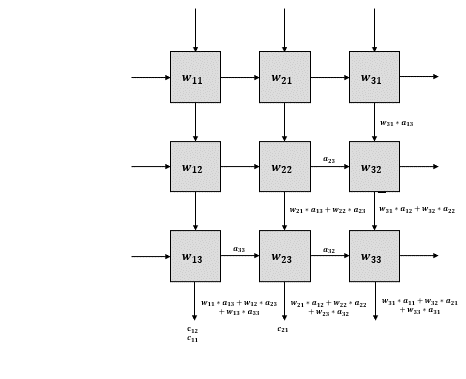
\includegraphics[height=4.1cm]{bench/img/sys_7.png}}%
\only<4>{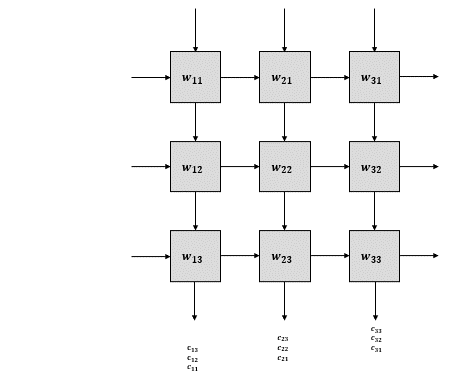
\includegraphics[height=4.1cm]{bench/img/sys_10.png}}\\[2pt]
{\tiny Weight-stationary dataflow: one operand fetch feeds a whole row.}
\end{center}
\end{minipage}

\end{frame}
